\chapter{绪论}
\label{cha:intro}

\section{引言}

自万维网创始人Time Berner-Lee于1998年提出语义万维网的概念\cite{berners1998semantic},语义网的发展逐渐受到业界人士的广泛关注。语义万维网是万维网的扩展,其数据带有一定的语义信息,使得计算机可自动理解并处理各数据直接的联系,从而促进人类与计算机之间的相互合作。
为了实现语义万维网的远景,万维网联盟(W3C)于2007年2月提出Linked Open Data概念,并于之后启动了LOD项目\footnote{\url{http://linkeddata.org/}},旨在为开放的语义数据集提供规范统一的组织规则。已有数据集都以URIs、RDF的形式公开在网上,并利用RDF链接关联不同数据源中的相关元素\cite{bizer2009linked}。
%根据LOD cloud diagram\footnote{http://lod-cloud.net/} 网页上显示,
统计\footnote{\url{http://lod-cloud.net/}}显示,
截止到2014年8月,LOD项目已发布了xxx个数据集,共含有xxx个RDF三元组。万维网上发布的链接数据为语义网数据规范提供了示例,是计算机处理语义的基础,推动了知识共享,对语义网的发展起着举足轻重的作用。相信随着LOD项目的推广,还会有更多来自不同领域,不同语言的数据集发布出来。

在LOD项目中,有一些广为人知的开放数据集,如跨领域的YAGO\cite{suchanek2007yago,suchanek2008yago,hoffart2013yago2,mahdisoltani2014yago3},DBpedia\cite{auer2007dbpedia,bizer2009dbpedia,lehmann2015dbpedia},FreeBase \cite{bollacker2008freebase},Wikidata\cite{vrandevcic2014wikidata,erxleben2014introducing},限定领域的如电影领域的LinkedMDB\cite{hassanzadeh2009linked}与学术领域下的DBLP。这些数据集融合了网页等数据源中的信息,将其结构化、标准化,便于查询与数据链接。

数据阵容逐渐壮大,基于语义数据集的应用也展露头脚。2012年谷歌提出将知识图谱\cite{singhal2012introducing}加入到搜索引擎中,在搜索体验上增加了语义理解功能,从而能返回直接的答案。因为“图谱”一词形象地展现点与边、知识与链接的关系,之后人们多以知识图谱表示从多个数据源中构成的大规模知识库。除了优化搜索,知识图谱在问答系统\cite{yih2015semantic,yang2014joint}、个性化推荐\cite{kaminskas2012knowledge}等领域也逐渐受到重视。大量语义关系信息使得依赖实体描述、语义推导而展开的新思维可以实现。

然而,在语义万维网与链接数据蓬勃发展的同时,中文知识依然匮乏。DBpedia基于维基百科构建,横跨包括电影、人物、地理等在内的多个领域,囊括英语、德语、法语、日语等97个语言版本,它因涉及内容广泛、结构完善,被视为链接数据的中心,目前包含24.6亿以上的三元组,然而DBpedia包含的中文知识屈指可数。另一个广受关注的知识库YAGO,在第三版本YAGO3中通过维基百科加入了德语、法语、意大利语等多国语言信息,但依然没有中文知识在其中。Wikidata由维基媒体基金会支持,完全基于维基百科源数据建立,含有一定数量的中文数据,但其中文知识数量受限于维基百科。目前为止,维基百科是全球最大的知识存储库。它建立于2001年,截止到2016年,已经涵盖了288种语言下的共2000多万条词条。图\ref{fig:wiki-stat}, 显示截止到2016年3月维基百科中几个主要语言的词条数量,当前中文词条仅有86万,仅为英文词条507万的约六分之一。由此可见,单纯基于维基百科建立知识库,在知识量上会受百科原有数据的限制,而中国用户在维基百科的参与度不高,中文知识的匮乏直接导致中文知识库创建困难,中文资源问题亟待解决。

\begin{figure}[H] % use float package if you want it here
  \centering
  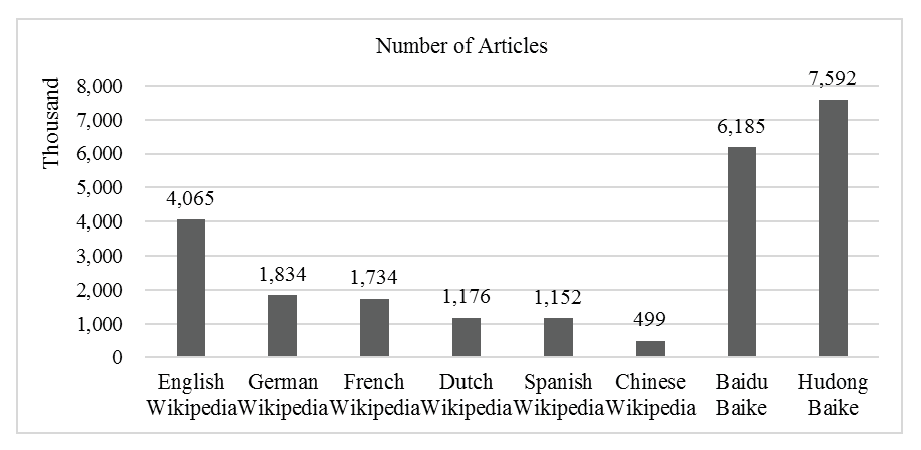
\includegraphics[width=0.8\columnwidth]{fig_stat}
  \caption{几个主要百科词条数量分布情况}
  \label{fig:wiki-stat}
\end{figure}

事实上,国内存在一些知名的通用领域的商业化百科全书,如百度百科\footnote{http://baike.baidu.com/}与互动百科\footnote{http://www.baike.com/},这些在线百科经过数以万计的人员撰写修改,已经形成很大规模,并存有丰富的中文知识。其中百度百科作为目前中国最大的开放式网络百科全书,收录了许多特色词条,因为参与编辑的人数多,编辑方式相对自由等原因,信息也更为全面。截止到2016年1月已收录词条超过1,313万条,远超过维基百科的中文词条数量。互动百科也有1430万个词条。如果能融合两个中文百科的信息,平衡中英文知识量级就可能实现。

国内切实存在一些商业化的中文知识库,如搜狗“知立方”和百度“知心”,它们都是以人性化搜索、个性化推荐为出发点所建立的知识图谱产品。研究领域也有Zhishi.me\cite{niu2011zhishi} 等中文知识库。然而,随着开放链接的增多,人们发现单语言数据集已经不能满足语义万维网知识融合,知识共享的特点。除了更好的融合多语言知识,跨语言链接还用来辅助机器翻译\cite{niehues2011using}、跨语言信息检索\cite{giang2015building}等。然而因为维基中文知识匮乏,中英文难以对齐等原因,中英文的跨语言链接还很少。

为解决中文知识匮乏问题,我们构建的大规模跨语言知识图谱XLore,充分利用最大的中、英文异构在线百科丰富的信息,即结合了中英文维基、百度百科、互动百科的知识,将词条、分类与信息框分别抽象成知识库中的实例、概念、属性,并利用维基的语言链接信息与跨语言链接扩展方法\cite{wang2012cross},添加双语知识的\textit{SameAs}关系,成功将双语语义信息融合在一起,为中英文知识共享打下了基础。

\section{挑战}

虽然目前知识图谱的构建已经有大量实践成果,我们的跨语言知识库XLore也在提供了一定中英文对齐知识,但知识库的完善,跨语言知识的增多,依然存在很多问题亟待解决。

本体作为知识库的骨架,其准确性与完整性非常重要。通常本体包含概念与属性,概念是对一些相似事物抽象出的类别,属性对事物特性进行描述。在RDF的定义中,有一些已定义的核心属性,如Rdf:type建立了实例与概念的instanceOf关系,也可以自定义属性。DBpedia有7000多个自定义属性,以\textit{http://nl.dbpedia.org/property}的形式定义。

基于百科构建的知识库,通常会通过词条信息框补充属性。信息框是一个词条的脸面,它包含了该词条的基本的、重要的信息,读者通过阅读信息框,就可以了解关于词条大部分重要内容。信息框中的属性是对相应实体的特性的描述,可以认为它是实例的自有属性,由此为本体设立的自定义属性可达上万个。哪些属性可描述同一类实体?同一表达形式的属性是否表达着唯一含义?概念下与属性要如何准确地描述本体?这些问题的解决,对构建一个准确、可用的知识库,起着重要作用。

在跨语言知识库构建过程中,本体对齐是核心关注点。维基百科提供了跨语言的词条链接,大部分跨语言知识库,如DBpedia、YAGO,都利用此链接集合匹配中英文实例与概念。但是,维基百科没有直接提供属性跨语言信息,并且其公开的数据文件中,也不含有可用信息框属性对齐关系。基于信息框的自定义属性链接的缺失,使得基于百科的跨语言本体在属性阶层无法匹配,知识库骨架无法形成。

据最新统计,截止到2016年2月,英文维基带有信息框的词条数量约是中文维基9倍,中文维基带有信息库的词条数量约为总词条数量的1/4。当前如果仅仅依靠维基百科获得属性对齐关系,必然会受到维基中英文知识数量不平衡的局限。

如何获取更多的属性跨语言链接?引入其他数据源进行补充依然是可行方法之一。然而因为异构百科在属性表示方面的迥异,编辑规则不一致,从标签文本角度出发是很片面的,即使在同语言情况下,也有很多相同属性不能直接对齐。比如中文维基使用\textit{制片商},百度百科使用\textit{出品公司}作为电影制作公司属性的标签,中文维基常有\textit{旁白}、\textit{配乐作品}等百度百科不使用的属性,等等。充分利用多源信息对知识的查漏补缺、错误修正有很大贡献,但面临的问题也有所增多。

此外,异构百科对于属性的领域界限划分模糊不清,维基百科中,信息库模板很好的给定了描述一类实体的属性集合。其他百科如百度百科,不包含模板信息。面对无规则无限制的杂乱属性集,如何准确定义概念属性,制定受认可的、特定领域下的模板,从而更好的为属性对齐服务,是我们需要考虑的难题。

属性的分析,对准确地描述本体、构建知识库起着重要作用。据我们所知,当前还没有中英文知识库对属性有过全面的分析与处理。XLore中虽然含有来自四个百科数据源的约6万个属性,但并没有进行进一步的跨语言对齐处理。如何处理异构百科的跨语言属性对齐,以及其衍生的一系列问题,从而完善我们的知识库,是当前亟需解决的问题。

基于知识库中属性的重要性,本文工作对百科的信息框属性进行了概念定义、同一查找、跨语言对齐等研究,力求获得更准确的本体框架,以及发现更多的跨语言链接。

\section{主要工作}
本节对文章涉及的主要工作进行初步的描述:从准确构建基于百科的知识库本体的目标出发,提出概念属性,在百科内尝试解决概念属性的生成、跨语言对齐等问题,以扶助构建跨语言本体,提高中英文信息的融合度。另外从知识库应用的角度出发,搭建展示系统与实体接口。本节根据之前提出的挑战,对涉及到的研究点进行了概括。

\subsection{维基百科概念属性生成}
针对本体中概念下的属性集合问题,我们定义概念属性,来表征某概念下一类实体的特性。维基百科中具备的信息框模板,对特定领域内实体的描述进行了规范,囊括领域范围内的属性集合。通过分析信息框模板,可以获得一系列概念属性。我们获取了维基百科大部分概念属性,该结果可覆盖维基中90\%以上的词条的信息框,为后续对概念属性的进一步研究打下了良好基础。

{\heiti 问题定义:} 给定一种语言的维基百科$W$,通过分析模板$T$,取得一系列概念$C$,以及相关的概念属性$\mathbb{P}_C=\{P{c_i}|i=1,2,...j\}$。

\subsection{异构百科跨语言属性对齐}
不同于大多数的跨语言属性对齐研究,本文将属性定义为概念属性,并同时进行百科异构性的分析,即对属性的研究建立在维基百科与百度百科两个异构百科上。结构与语言的双重障碍,为属性对齐的研究增加了难度。为尽可能达到结构上的统一,我们对无模板的百度百科属性集合生成概念属性,形成领域下的模板,并将属性对齐问题限定在概念领域范围下,同时利用中文维基为英文维基与百度百科搭桥引线,获取更多关联信息。

总结来说,本问题通过四个步骤解决并优化,分别为:1)生成百科概念属性模板,2)同语言对齐与相似属性合并,3)跨语言种子集合生成,4)跨语言属性对齐。

{\heiti 问题定义:} 给定两个中英文异构百科$W_{e}$与$W_{z}$,在限定领域$C$下,获得该属性集合,生成领域模板${T_{C}}$,并在该模板下,聚集相似属性组成超级属性$sp$,对齐跨语言属性$sp_{e} \Leftrightarrow sp_{z}$。

\subsection{中英文跨语言知识库的构建与应用}
本文提及的知识库系统XLore,其构建初衷是为解决中文知识匮乏问题,提高知识融合度与共享率,面对当前多语言在线百科与知识库中中英文信息极度不平衡的现状,利用其他丰富的中文资源不失为一则良策。基于此我们将目光聚焦在国内信息最丰富的两大在线百科全书——百度百科与互动百科上,利用两大百科的词条页面信息、分类体系数据,并结合维基百科对外发布的数据存储文件,抽取结构化信息,经过一系列的知识处理流程,获得语义信息,构成跨语言知识库XLore。图\ref{fig:xlore-procedure}为XLore的构建流程。

\begin{figure}[H]
  \centering
  \includegraphics[width=0.8\columnwidth]{xlore-procedure}
  \caption{知识图谱XLore构建流程}
  \label{fig:xlore-procedure}
\end{figure}

值得一提的是,我们对XLore知识库的应用层次上也进行了尝试,主要体现在支持数据访问的在线系统XLore.org,以及提供实体语义信息的API接口,该接口支持限定领域查询与通用领域实体查询。

\subsection{主要贡献}
本文提出了一种概念属性生成与领域跨语言属性对齐的方法,并利用对齐结果与四个百科数据源的抽取结果,构建通用领域的中英文知识库XLore,其中主要贡献列举如下:
\begin{enumerate}[1)]
\item {\heiti 概念属性的定义与生成,} 工程抽取与算法计算相结合,提取出英文维基百科与百度百科两个异构百科下的信息框属性关系。包括百科下属性模板生成,与限定领域下的中英文属性匹配。该方法在构建大规模知识库过程中,对于从多语言的异构数据源生成对齐的shema有一定的贡献。
\item {\heiti 异构百科下的跨语言概念属性对齐,} 工程抽取与算法计算相结合,提取出英文维基百科与百度百科两个异构百科下的信息框属性关系。包括百科下属性模板生成,与限定领域下的中英文属性匹配。该方法在构建大规模知识库过程中,对于从多语言的异构数据源生成对齐的shema有一定的贡献。
\item {\heiti 构建跨语言知识库XLore,并提供多元化的数据展示与应用接口,}前者分别从一般用户与专业用户的不同角度,给出搜索框查询与SPARQL查询两种知识访问方式;后者考虑知识库的应用场景,提供基于RestFul的实体访问API,对给定文本进行实体分析与排歧,返回实体语义信息,实现了一定应用价值。
\end{enumerate}

\section{论文组织}

本文通过绪论、研究现状、基于维基百科概念属性生成、基于异构百科的跨语言属性对齐、中英文知识库XLore系统与应用接口、总结与展望共6个章节来组织全文内容,其章节关系与结构组织如图\ref{fig:organization}所示:

\begin{figure}[ht] % use float package if you want it here
  \centering
  \includegraphics[width=0.66\columnwidth]{organization}
  \caption{论文组织结构图}
  \label{fig:organization}
\end{figure}

第 1 章为绪论,对本文的研究背景进行描述,提出可能的挑战,并概要地介绍工作内容,交待论文的主要贡献及文章组织结构;

第 2 章为研究现状,介绍当前构建的跨语言知识图谱的发展情况,列举当前广为人知的多语言与中文单语言知识图谱,并介绍其构建技术;并对跨语言本体对齐研究现状进行描述,包括schema对齐,属性对齐等;此外从知识库应用角度,介绍实体链接的常见研究点。

第 3 章详细分析了维基百科的信息框编辑规则,对数据文件中的模板给出了分类与处理方法,由此定义概念属性,并以覆盖大部分词条描述为目标,借由模板生成概念属性;

第 4 章说明了基于异构百科的跨语言属性对齐流程。首先通过观察与抽取百科中的模板与属性,提出异构百科属性研究的种种难点,之后为百科属性集合提取概念属性模板,并实现在特定领域下,同语言相似属性的对齐与跨语言属性链接;

第 5 章简要介绍了基于多源异构在线百科,构建跨语言知识图谱XLore的过程,重点展示了为XLore搭建的可视化系统与数据访问接口,从实际应用角度展示该知识图谱的结构化与可用性;

第 6 章对本文提出的跨语言属性对齐与知识图谱构造研究工作进行了总结和展望,分析了不足之处,为下一步研究提出了新的建议和意见。

%\subsection{页面元素介绍}
%
%四个在线百科的词条页面在布局上很相近。通常,一个词条页面可以贡献两种带有潜在语义信息的元素,分别为所属分类信息与词条内容信息。分类信息包含负分类、自分类及其上下位关系信息。 图xxx是互动百科分类页面的截图。
%
%一个词条页面描述了一个显示中的实例。这些实例的丰富的信息由一个或多个经过专业认证的编写者们创建或修改,一般其信息内容都一定的可考证依据。另外,一篇词条可能归属于一个或多个分类。词条自带的实例内容、其与其他词条的关系,以及它所属的类别,都在构建知识库时起着重要作用。一般来说,一篇词条页面中,有五种元素可以被利用:
%
%{\heiti 标题:} 词条标题,即其所表征实体的名称,可以作为区分不同实体的表识,其内容在同一百科中是唯一、不可重复的。维基百科、互动百科、百度百科都对重名的不同实体做消歧处理,并在标题上表现出来,比如。。。
%
%{\heiti 摘要:}摘要是实体的一端剪短的简介,通常包含该实体的重要信息。一般是页面正文的第一段话。
%
%{\heiti 信息框:}一部分词条中带有信息框。信息框是一个表格形式,内含属性-属性值对,带有实体重要的属性信息。从信息框中可抽取主语-属性-属性值的三元组格式的结构化信息,其中主语即为该词条所表征的实体。
%
%{\heiti 链接:}词条文本中的超链接部分,是另一个词条的入口,点击即可进入对应词条的页面。它表征该词条与百科中其他词条的关系,是构成知识库中实体与实体关系的重要信息。
%分类:一个词条所属分类一般在该词条页面的底部一行显示,已标签或超链接的形式渲染。一个词条可能归属于一个或多个分类,表征知识库中的is-a关系。
%
%图XX是一篇中文维基的词条页面
%
%需要提到的一点:维基百科中页面内容的组织是遵从于维基模版制成的。此模版对词条编辑时,所要遵循的内容、结构等信息进行了约束。比如xxx,xxx。信息框的填充也从模板中产生。比如:词条 星际穿越根据模板Infobox film来编写,按规定来说,电影词条的信息框信息都应根据此模版来编辑。信息框模板带有电影领域公认的、常用的属性集合。
%
%除此之外,维基百科中,大部分词条的页面左边栏中,还提供了跨语言链接,该链接指向其他语言下该实体的词条页面。利用这些人工构建的跨语言信息,我们可以获得初步的跨语言链接集合。
%
